% Section content template for individual Educative lessons
% This file contains the actual content for a specific section
% Generated from Educative API section content

% Section: Activity Diagram for the Vending Machine
% Section ID: 6512840561393664
% Section Slug: activity-diagram-for-the-vending-machine
% Generated: 2025-12-11T20:26:23.479651

Activity diagrams are a great way to visualize the flow of messages from one activity to another in the system. We can create different activity diagrams for our vending machine. In this lesson, we will create an activity diagram for purchasing a product from the vending machine.

\subsection{Product purchase from the vending machine}\label{9LPU_Aw11EbVffW-Vcal3}
\\
The following are the states and actions involved in this activity diagram.

\subsubsection{States}\label{hu_53AizBHxaqt8GSqc6F}
\\
\textbf{Initial state:} The customer inserts money into the vending machine.
\\
\textbf{Final state:} The customer receives the desired product.

\subsubsection{Actions}\label{hwPLF3KrHnbB9-jrIeyHh}
\\
The customer interacts with the vending machine and inserts money. The customer selects their desired product. If that product is available, they get the product and the change. Otherwise , the system shows a message of product unavailability and asks the customer to select another product.
\\
Based on the order above, the activity diagram of a product purchase from the vending machine is shown below:

\begin{figure}[htbp]
 \centering
 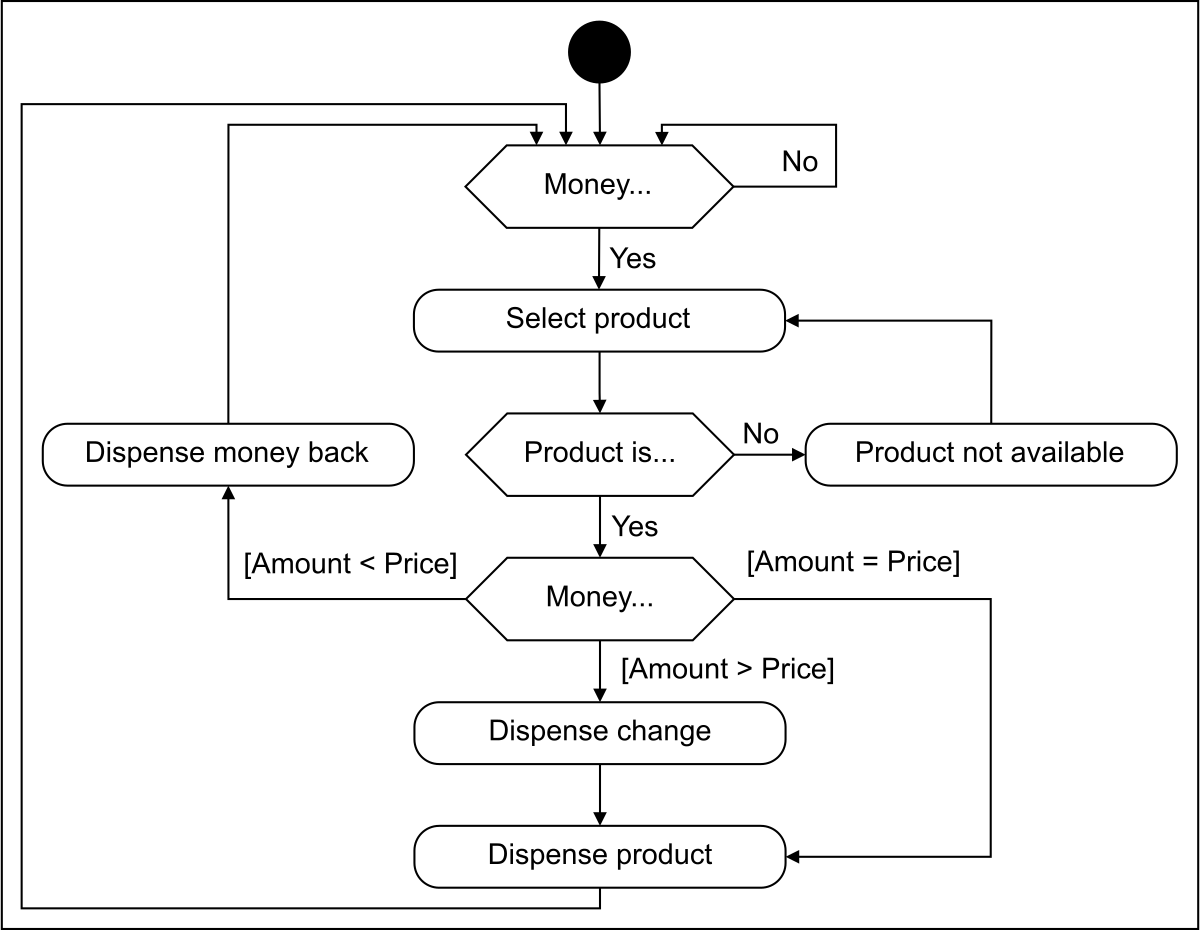
\includegraphics[width=0.5\textwidth]{Images/chapter_11/section_6512840561393664/5476016460136448.png}
 \caption{The activity diagram for the product purchase from the vending machine}
\end{figure}

We've looked at the activity diagram of our vending machine. In the next lesson, we will present the code for our designed classes in some of the most popular languages.

% End of section content